\documentclass[iop]{emulateapj}
\usepackage{color}
\usepackage{natbib}
\usepackage{amsmath}
\bibliographystyle{apj}

\newcommand{\vdag}{(v)^\dagger}
\newcommand{\myemail}{eogorma@tcd.ie}

\shorttitle{BETELGEUSE'S WIND ACCELERATION REGION}
\shortauthors{O'GORMAN ET AL.}

\begin{document}

\title{MULTI EPOCH SPATIALLY RESOLVED RADIO OBSERVATIONS OF BETELGEUSE'S WIND ACCELERATION REGION}


\author{Eamon O'Gorman\altaffilmark{1}, Graham M. Harper\altaffilmark{1}, Alexander Brown\altaffilmark{2}, and Anita M. S. Richards\altaffilmark{3}}
\altaffiltext{1}{School of Physics, Trinity College Dublin, Dublin 2, Ireland}
\altaffiltext{2}{Center for Astrophysics and Space Astronomy, University of Colorado, 389 UCB, Boulder, CO 80309, USA}
\altaffiltext{3}{Jodrell Bank Centre for Astrophysics, School of Physics and Astronomy, University of Manchester, Manchester M13 9PL, UK}

%\email{eogorma@tcd.ie}
%\email{graham.harper@tcd.ie}
%\email{alexander.brown@colorado.edu}
%\email{a.m.s.richards@manchester.ac.uk}


\begin{abstract}

Previous VLA observations have only spatially resolved the stellar atmosphere at 0.7\,cm but here we fully resolve the star at all wavelengths between 0.7 and 6.1\,cm. New multi-epoch e-MERLIN data are urgently required.

\end{abstract}

\keywords{Radio continuum: stars --- Stars: supergiants --- Stars: individual ($\rm{\alpha}$ Ori) --- Stars: mass-loss --- Stars: winds, outflows}

\section{INTRODUCTION}
The problem with early M supergiants and introduce Betelgeuse

The wind acceleration region importance and thermal free-free as a probe

Previous radio observations (earlier VLA in agreement with ALfven models, skinner, lim, richards)

Why this paper, i.e. looking for evidence of emerlin



\section{OBSERVATIONS AND DATA REDUCTION}

\begin{deluxetable*}{lcccccccc}
\tabletypesize{\scriptsize}
%\tablecolumns{6} 
%\tablewidth{0pt} 
\tablecaption{Multi Epoch VLA A-Configuration Plus Pie Town Link Observations of Betelgeuse.}
\tablehead{\colhead{Date}						&
			\colhead{Wavelength}			    &
           	\colhead{Restoring Beam}            &
           	\colhead{Image rms}            		&
           	\colhead{$\theta _{\mathrm{maj}}$}  &
			\colhead{$\theta _{\mathrm{maj}}/\theta _{\mathrm{min}}$}	&
           	\colhead{P.A.}  &
          	\colhead{$F_{\nu}$}  &
           	\colhead{$T_{b}$}  \\
	\colhead{}		                			& 
	\colhead{(cm)}                         		& 
	\colhead{(mas $\times$ mas)}   	&
	\colhead{(mJy/Beam)}                    	&
	\colhead{(mas)}   		    &
	\colhead{}   		    &
	\colhead{(deg)}   		    &
	\colhead{(mJy)}   		    &
	\colhead{(K)}		}
\startdata
		 2004 Oct 21,30  & 0.7 & $39\times 26$ & 0.37	& $99\pm 3$ & $0.93\pm 0.04$& $92\pm 20$ &$28.67\pm 0.53$ & $2940\pm 170$\\
		 				 & 1.3 & $80\times 42$ & 0.09   & $121\pm 2$& $\dots$ & $\dots$& $13.88\pm 0.10$& $3140\pm 80$\\
						 & 2.0 & $121\times 91$ & 0.08  & $158\pm 6$& $\dots$ & $\dots$ & $7.23\pm 0.15$& $2270\pm 130$ \\
						 & 3.6 & $208\times 126$ & 0.02	& $215\pm 7$& $0.87\pm 0.04$ & $162\pm 7$& $3.34\pm 0.03$& $2110\pm 110$\\
						 & 6.1 & $377\times 264$ & 0.02	& $315\pm 30$& $0.59\pm 0.13$ & $173\pm 10$ & $1.55\pm 0.04$& $1140\pm 160$\\
						 & 20.5& $1262\times 889$ & 0.03& $\le 889$ & $\dots$ & $\dots$ &$0.25\pm 0.03$ &\\
\hline
\rule{-2.6pt}{2.5ex}  2003 Aug 10,12 & 0.7 		& &	& $103\pm 4$& $0.89\pm 0.06$ & $104\pm 16$& $28.05\pm 0.84$& $2760\pm 230$ \\
									 & 1.3		& &	& $122\pm 5$& $\dots$& $\dots$& $11.20\pm 0.24$& $2490\pm 150$\\
									 & 2.0		& &	& $132\pm 10$& $0.87\pm 0.10$& $11\pm 27$& $5.88\pm 0.17$&$3040\pm 360$\\
									 & 3.6		& &	& $193\pm 7$& $0.73\pm 0.06$ & $152\pm 7$& $2.80\pm 0.04$&  $2610\pm 170$\\
									 & 6.1 		& &	& $209\pm 49$& $\dots$ & $\dots$& $1.22\pm 0.04$&$2040\pm 680$ \\
					                 &20.5		& &	& $\dots$& $\dots$ & $\dots$& $0.26\pm 0.03$& \\
\hline
\rule{-2.6pt}{2.5ex}  2002 Apr 12,13  & 1.3 		& &	&$134\pm 9$ & $0.76 \pm 0.07$& $36\pm 10$& $8.96\pm 0.24$& $2170\pm 250$\\
							& 2.0		& &	& $166\pm 16$& $0.63\pm 0.10$&$41\pm 11$ & $5.32\pm 0.23$& $2420\pm 450$ \\
							& 3.6		& &	& $234\pm 9$& $0.73\pm 0.05$& $40\pm7$& $2.66\pm 0.04$& $1690\pm 110$\\
							& 6.1 	& &	& $\dots$ & $\dots$& $\dots$& $\dots$& $\dots$\\
							& 20.5	& &	& $\dots$ & $\dots$ & $\dots$& $0.38\pm 0.06$& \\
\hline
\rule{-2.6pt}{2.5ex}  2002 Feb 17,18 & 1.3 		& &	&$120\pm 4$ & $0.91\pm 0.04$& $30\pm 13$&$10.87\pm 0.17$ & $2750\pm 140$\\
									& 2.0		& &	&$140\pm 13$& $\dots$& $\dots$&$5.38\pm 0.22$ & $2150\pm 300$\\
									& 3.6		& &	&$199\pm 8$ & $\dots$& $\dots$ & $2.85\pm 0.04$& $1830\pm 110$\\
									& 6.1 		& &	& $\dots$& $\dots$& $\dots$& $\dots$& $\dots$\\
									& 20.5		& &	& $\dots$& $\dots$& $\dots$& $0.30\pm 0.05$& \\
\hline
\rule{-2.6pt}{2.5ex}  2001 Jan 02  & 1.3 		& &	&$124\pm 0.02$ & $0.92\pm 0.02$& $40\pm 8$& $12.58\pm0.08$& $2920\pm 70$ \\
 		 2000 Dec 23 & 0.7		& &	&$98\pm 2$ &$0.92\pm 0.02$ &$0\pm 7$ & $29.02\pm 0.30$& $3070\pm 100$\\
\hline
\rule{-2.6pt}{2.5ex}  1998 Mar 29,30 & 0.7 		& &	& $104\pm 6$& $0.88\pm 0.07$& $118\pm 20$& $18.19\pm 0.73$& $1770\pm 180$ \\
									 & 1.3		& & 	& $157\pm 8$ & $0.61\pm 0.06$& $46\pm 6$&$10.99\pm 0.31$ & $2420\pm 250$
\enddata
\tablenotetext{}{Notes.- Restoring beam size obtained using uniform weighting. The P.A. is measured in degrees east of north. }
\label{tab:tab1}
\end{deluxetable*}



The data were imaged within the Common Astronomical Software Application  \cite[CASA;][]{2007ASPC..376..127M} package.\\
The xxx uvmodelfit was used while bounding the axis ratio between 0 and 1, and the position angle between 0 and 180. \\
Phase center was found using Reid \& Menton\\

\section{RESULTS} 
\subsection{Visibilities} 
\subsection{Radio Maps} 



\section{DISCUSSION}
\subsection{Radio Flux Density Variability} 
see Reid \& Menton 1996 conf proceedings\\
see Drake conf proceedings\\
e-MERLIN flux is concentrated\\
see Harper\_variability. ps\\
does flux go up as ang diam go up

\subsection{Structure of Wind Acceleration Region} 
Thermal structure (Lim vs vs Ours vs e-MERLIN)\\
see Reid \& Menton 1996 conf proceedings\\
Harper model

\subsection{Where are the Hotspots?}

No sign of hotspots (see Harpers pie town proceedings )




\begin{figure*}
\mbox{
\includegraphics[trim = 30mm 90mm 50mm 80mm, clip,scale=0.55]{/home/eamon/pietown/paper/figs/nature_fig.ps}
\includegraphics[trim = 0mm 50mm 20mm 58mm, clip,scale=0.4,angle=90]{/home/eamon/pietown/paper/figs/vla_q_2000.ps}
\includegraphics[trim = 0mm 0mm 20mm 58mm, clip,scale=0.40,angle=90]{/home/eamon/pietown/paper/figs/vla_q_2004.ps}
}
\caption{VLA A-configuration maps of Betelgeuse at 0.7\,cm. }
\label{fig:fig5}
\end{figure*}




\section{CONCLUSIONS}
 


\acknowledgments
The data presented in this paper were obtained with the Karl G. Jansky Very Large Array (VLA) which is an instrument of the National Radio Astronomy Observatory (NRAO). The NRAO is a facility of the National Science Foundation operated under cooperative agreement by Associated Universities, Inc. We wish to thank the NRAO helpdesk for their detailed responses to our CASA related queries. This publication has emanated from research conducted with the financial support of Science Foundation Ireland under Grant Number SFI11/RFP.1/AST/3064, and a grant from Trinity College Dublin.

{\it Facilities:} \facility{VLA}.



\bibliography{references}

\end{document}
